% Resumen ejecutivo Galaxy Vision. Basado en la plantilla institucional proporcionada.
\documentclass[letterpaper,11pt]{article}
\usepackage[utf8]{inputenc}
\usepackage[T1]{fontenc}
\usepackage{lmodern}
\usepackage[spanish,es-tabla]{babel}
\usepackage[margin=2.5cm,headheight=52pt,headsep=0.3cm]{geometry}
\usepackage{setspace}\setstretch{1.15}
\usepackage{graphicx,booktabs,tabularx,array}
\usepackage[font=small,labelfont=bf]{caption}
\usepackage{csquotes,xcolor,enumitem}
\usepackage[hidelinks]{hyperref}
\usepackage[style=apa,backend=biber]{biblatex}\addbibresource{referencias.bib}
\usepackage{fancyhdr}
\pagestyle{fancy}\fancyhf{}\renewcommand{\headrulewidth}{0pt}\fancyfoot[C]{\thepage}
\fancyhead[L]{
\includegraphics[height=1.2cm]{logo.jpeg}}
\newcommand{\metric}[2]{\textbf{#1}\\[-2pt]{\footnotesize #2}}
\setlength{\parindent}{1em}\setlength{\parskip}{2.5pt}
\captionsetup{skip=3pt}
\begin{document}
\thispagestyle{fancy}
{\LARGE\bfseries Galaxy Vision: clasificación morfológica de galaxias con aprendizaje automático\par}
{\large Resumen ejecutivo para el Instituto de Astronomía de la UNAM\par}
\vspace{3pt}
{\footnotesize \textbf{Integrantes:} Alexander Carreño, María Rabelero y Julio Ricardo Velázquez \quad
\textbf{Sponsors:} Dr. José Antonio Vázquez Mata y Dr. Héctor Manuel Hernández Toledo \quad
\textbf{Fecha:} 17 de noviembre de 2026}\par
\vspace{4pt}
\textbf{Problema y solución.} La clasificación morfológica de galaxias se realiza principalmente mediante inspección visual; a gran escala consume tiempo especializado y puede variar entre clasificadores. El reto crecerá con los grandes volúmenes de imágenes del Vera C. Rubin Observatory (LSST), cuya explotación científica requiere métodos reproducibles y escalables. Galaxy Vision explora una clasificación binaria inicial —galaxias tempranas (Ttype $\leq 0$) y tardías (Ttype $\geq 1$)— combinando imágenes, espectros MaNGA y poblaciones estelares STARLIGHT. La propuesta es usar el modelo como apoyo para priorizar y organizar la revisión científica, no como sustituto del criterio experto.\par
\textbf{Desempeño experimental.} Los experimentos comparten una partición de prueba de 1,403 galaxias. Los resultados muestran que las imágenes son la modalidad más fuerte; la fusión multimodal presenta una mejora pequeña y todavía no concluyente frente a modelos visuales. En la variante M2 por tokens se reporta AUC-ROC de 0.9666 y exactitud entre 89.9\% y 90.2\%; la CNN RGB entrenada en CPU alcanza AUC 0.9634 y exactitud 90.09\%. Las poblaciones STARLIGHT por sí solas alcanzan AUC 0.8949 y exactitud 83.75\%, mientras que una arquitectura espectral optimizada llega a AUC 0.917. AUC mide la capacidad de ordenar correctamente casos de ambas clases; no equivale a una tasa de acierto. La diferencia M2–ResNet-18 es de aproximadamente 0.0033 y se basa en una semilla y un solo split, por lo que debe confirmarse con repeticiones independientes.\par
\begin{center}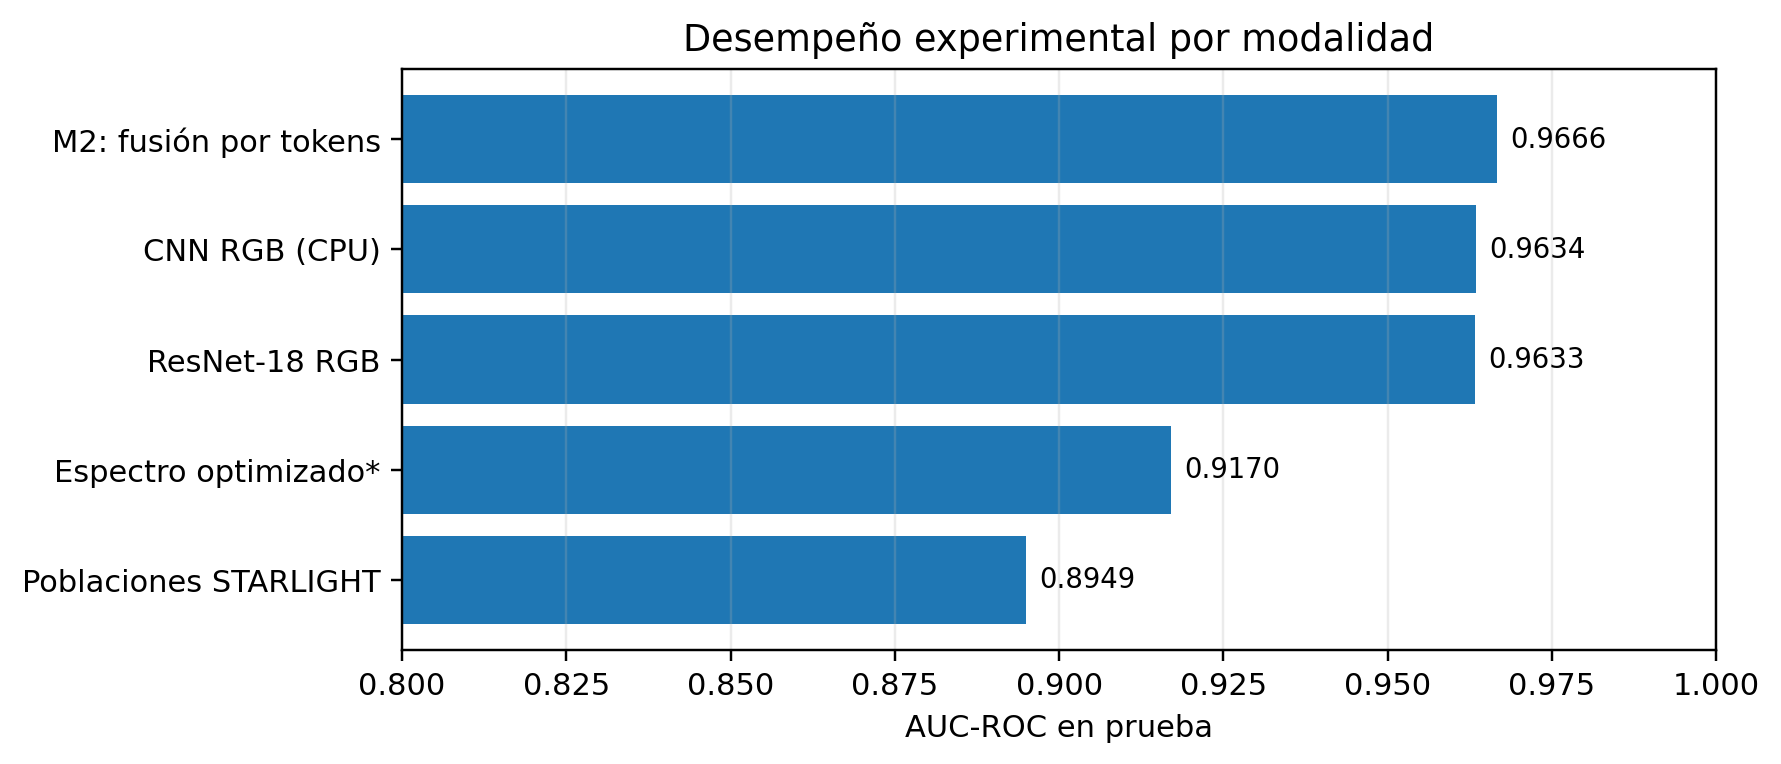
\includegraphics[width=0.84\linewidth]{figura1_auc.png}\end{center}
\captionof{figure}{Comparación de AUC-ROC reportada en el análisis experimental. *La arquitectura espectral optimizada se reporta como experimento separado de la ablación. Fuente: análisis de experimentos del repositorio Galaxy Vision.}\label{fig:auc}
\textbf{Beneficios para la organización.} El beneficio principal esperado es ampliar la capacidad de análisis de catálogos y reducir la dependencia de clasificación visual individual, especialmente como etapa de preselección y control de calidad. También puede aportar reproducibilidad, trazabilidad de predicciones, criterios homogéneos de priorización y una base técnica reutilizable para adaptar modelos a nuevas muestras del LSST \parencite{galaxyproject}. Estos beneficios son potenciales: todavía no existe una operación institucional ni una línea base de galaxias clasificadas por Galaxy Vision \parencite{galaxyablacion}.\par
\textbf{Beneficios cuantificables mensuales.} Con la información disponible no es responsable asignar horas ahorradas, MXN ahorrados, errores evitados ni volumen mensual: no se ha iniciado clasificación institucional y no se conoce el tiempo humano por galaxia ni el rendimiento de inferencia en el equipo objetivo. Por ello, estos indicadores se reportan como \emph{pendientes de medir} y se definen sus fórmulas en el Anexo A. No se presentan como ahorros realizados.\par
\textbf{Inversión y costo total de propiedad (TCO).} El prototipo se ha trabajado en computadora personal sin GPU dedicada. En el escenario base no se presupone compra de hardware, licencias ni contratación; por tanto, el desembolso incremental en efectivo podría ser \$0 MXN si se mantienen los recursos existentes y las dependencias son gratuitas. Esto \emph{no} representa un TCO completo: faltan horas de desarrollo y soporte valorizadas, consumo eléctrico, almacenamiento, conectividad y cualquier servicio institucional. La selección debe priorizar utilidad y costo total, no solo una métrica aislada \parencite{baccarin2020}. El TCO de 12 meses queda \textbf{no estimable con la información actual}; el Anexo B presenta los rubros y la forma de cotizarlos.\par
\textbf{Recomendación al sponsor.} Autorizar una fase piloto acotada, sin compromiso inmediato de despliegue productivo ni compra de GPU. El piloto debe medir tiempo de inferencia y entrenamiento en CPU, desempeño por clase, calibración y errores en una muestra externa revisada por especialistas. Solo después de ese benchmark deberá decidirse si conviene mantener CPU, usar infraestructura institucional o contratar cómputo acelerado.\par
\textbf{Riesgos y condiciones para avanzar.} (1) Etiquetas morfológicas inciertas, sobre todo cerca de Ttype 0–1: auditar una muestra con revisión experta y documentar desacuerdos. (2) Generalización limitada por una sola semilla y partición: repetir entrenamiento con varias semillas y validación externa. (3) Sobreajuste en ResNet-18 y fusiones: aplicar regularización, aumento de datos y monitoreo de brecha entrenamiento-validación. (4) Tiempo de cómputo en CPU: medir latencia y rendimiento por lote antes de fijar capacidad. (5) Cambio de distribución entre MaNGA y LSST: evaluar y recalibrar con datos representativos del nuevo observatorio antes de transferir el modelo \parencite{babic2021}.\par
\textbf{Transferencia y continuidad.} Entregar código fuente y notebooks, configuración y pesos de modelos, definición de etiquetas y particiones, resultados reproducibles, curvas y matrices de confusión, ficha de datos, registro de dependencias y guía operativa para preparar datos, ejecutar inferencia, interpretar probabilidades, revisar casos inciertos, registrar errores y reentrenar. La continuidad deberá quedar a cargo de un responsable técnico y un responsable científico designados por el sponsor.\par
\textbf{Declaración de uso de IA.} Se utilizó OpenAI (2026), ChatGPT (basado en GPT-6) [modelo de lenguaje grande], como apoyo para estructurar y revisar la redacción del resumen ejecutivo y para generar las gráficas de presentación a partir de métricas proporcionadas. Los autores verifican y asumen la responsabilidad final del contenido.\par
\printbibliography[title={Referencias}]
\clearpage
\appendix
\section*{Anexo A. Beneficios mensuales: indicadores y bases de cálculo}
Los siguientes indicadores son objetivos de medición para un piloto; no son beneficios observados. Para estimarlos se deberá fijar un periodo mensual, una muestra representativa y un protocolo de comparación con clasificación humana.
\begin{tabularx}{\linewidth}{p{3.2cm}p{3.0cm}X}
\toprule\textbf{Indicador} & \textbf{Unidad mensual} & \textbf{Base de cálculo y dato faltante}\\\midrule
Ahorro de tiempo & horas/mes & $N_m\times(t_h-t_{IA})/60$. $N_m$: galaxias procesadas/mes; $t_h$: minutos humanos por galaxia; $t_{IA}$: minutos de revisión humana por predicción. Medir ambos tiempos en piloto.\\
Productividad/capacidad & galaxias/mes & $N_m=\mathrm{tasa\_inferencias}\times\mathrm{horas\_disponibles}\times\mathrm{utilizacion}$. Medir inferencias/minuto en computadora objetivo y disponibilidad mensual.\\
Reducción de errores & errores/mes o \% & Comparar falsos positivos y falsos negativos contra etiquetas adjudicadas por especialistas; no usar accuracy de test como reducción de errores operativos.\\
Ahorro operativo & MXN/mes & Horas netas liberadas $\times$ costo laboral cargado por hora, menos costo mensual de cómputo, almacenamiento y soporte. Requiere costo laboral institucional.\\
\bottomrule
\end{tabularx}
\vspace{4pt}
\textbf{Supuestos que deben validarse:} (a) el sponsor define el volumen mensual objetivo; (b) se mide el tiempo de revisión humana, no solo la inferencia automática; (c) una predicción cuenta como útil solo después de establecer criterios de aceptación; (d) las etiquetas de referencia son revisadas por especialistas; (e) se reportan resultados por clase y por nivel de confianza.\par
\section*{Anexo B. TCO a 12 meses: desglose preliminar}
\begin{tabularx}{\linewidth}{p{3.0cm}p{2.6cm}X}
\toprule\textbf{Rubro} & \textbf{Estimación actual} & \textbf{Tratamiento para cotización}\\\midrule
Desarrollo & No estimable & Horas de ingeniería/ciencia de datos ya invertidas y horas adicionales para robustecer, documentar y probar; multiplicar por costo cargado/hora.\\
Implementación & \$0 MXN incremental supuesto & Escenario base con computadora personal existente y sin GPU. Incluir instalación, integración, capacitación y validación institucional si se requieren.\\
Operación & No estimable & Electricidad, almacenamiento, respaldo, mantenimiento, monitoreo, soporte y eventuales servicios de cómputo.\\
Hardware/GPU & \$0 MXN en escenario base & No se contempla compra. Cotizar GPU o nube únicamente si el benchmark CPU no satisface el volumen y plazo definidos.\\
Licencias/software & \$0 MXN supuesto & Confirmar licencias, cuotas y términos de uso de cada dependencia, dataset y servicio antes del piloto.\\
\midrule
\textbf{TCO 12 meses} & \textbf{No estimable} & $TCO=desarrollo+implementación+operación+hardware/licencias$. El desembolso incremental podría ser $0$ solo si no se contratan recursos ni servicios y se absorbe el trabajo como aportación en especie.\\
\bottomrule
\end{tabularx}
\vspace{4pt}
\textbf{Recomendación presupuestal:} aprobar primero un piloto con recursos existentes y un tope de gasto por definir. Solicitar presupuesto adicional solo con evidencia de latencia, volumen, costo de personal y necesidad de aceleración. Registrar por separado aportaciones en especie y desembolsos para no confundir costo económico con flujo de efectivo.\par
\section*{Anexo C. Riesgos, controles y criterios de salida}
\begin{tabularx}{\linewidth}{p{3.0cm}X X}
\toprule\textbf{Riesgo} & \textbf{Mitigación} & \textbf{Criterio de avance}\\\midrule
Etiquetas ambiguas o sesgadas & Auditoría estratificada, doble revisión y adjudicación experta, especialmente Ttype 0–1. & Acuerdo interevaluador y matriz de confusión documentados.\\
Variabilidad del modelo & Varias semillas, splits y validación externa sin fuga entre objetos. & Intervalos de confianza y desempeño estable por clase.\\
Sobreajuste & Regularización, augmentations y early stopping; comparar contra CNN compacta. & Brecha train/validación controlada y test externo consistente.\\
CPU insuficiente & Benchmark por tamaño de lote, memoria y tiempo total de entrenamiento/inferencia. & Cumplir el SLA científico que defina el sponsor.\\
Deriva MaNGA--LSST & Evaluar cambio de dominio, recalibrar y validar con imágenes representativas LSST. & Aprobación científica antes de uso sobre nueva población.\\
\bottomrule
\end{tabularx}
\vspace{4pt}
\begin{center}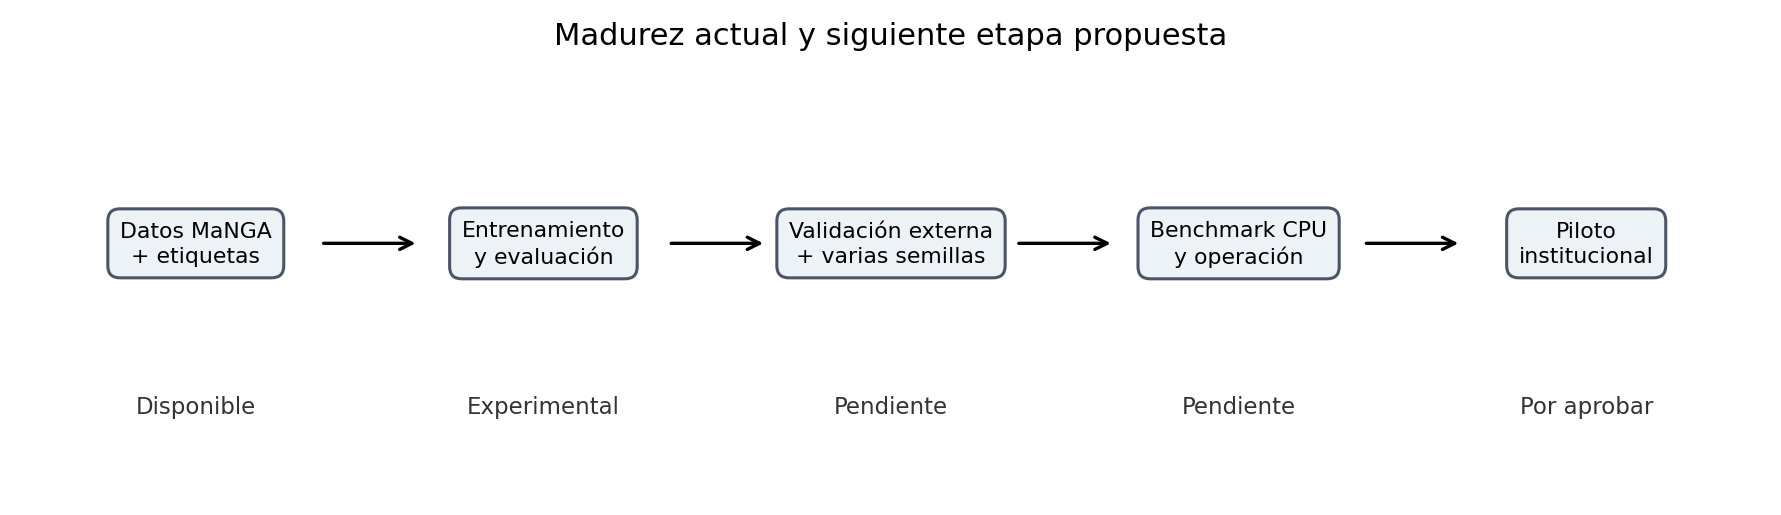
\includegraphics[width=0.96\linewidth]{figura2_madurez.png}\end{center}
\captionof{figure}{Estado de madurez y secuencia recomendada para pasar de experimentos a un piloto institucional. Fuente: elaboración del equipo a partir del estado actual del proyecto.}
\section*{Anexo D. Fuentes y notas metodológicas}
El documento de proyecto identifica la clasificación visual como cuello de botella ante catálogos grandes y plantea la preparación para LSST; también define la dicotomía Ttype temprana/tardía. El análisis de ablación informa que los experimentos comparten split train/validación/prueba (6,545/1,403/1,403), pero advierte que los resultados se basan en una semilla y un split. La fusión por tokens M0/M1/M2 obtuvo AUC 0.9660/0.9661/0.9666; las variantes no son distinguibles entre sí y la mejora frente a ResNet-18 es pequeña. La CNN de imágenes ejecutada en CPU registró 715 segundos por época, lo que refuerza la necesidad de medir cómputo en el equipo objetivo.\par
\end{document}
